\documentclass[conference]{IEEEtran}
\IEEEoverridecommandlockouts
% The preceding line is only needed to identify funding in the first footnote. If that is unneeded, please comment it out.
\usepackage[german]{babel}
\usepackage{amsmath,amssymb,amsfonts}
\usepackage[backend=biber,style=numeric,sorting=ynt]{biblatex}
\addbibresource{library.bib}
\usepackage{algorithmic}
\usepackage{graphicx}
\usepackage{tikz}
\usepackage{pgfplots}
\usepackage{textcomp}
\usepackage{pdfpages}
\usepackage[utf8]{inputenc}
\def\BibTeX{{\rm B\kern-.05em{\sc i\kern-.025em b}\kern-.08em
    T\kern-.1667em\lower.7ex\hbox{E}\kern-.125emX}}
\begin{document}

\title{Maschinelles Lernen in der Diagnostik einer Autismus-Spektrum-Störung bei Erwachsenen}

\author{\IEEEauthorblockN{Andreas Zinkl}
\IEEEauthorblockA{OTH Regensburg\\
Regensburg, Deutschland \\
andreas.zinkl@st.oth-regensburg.de}}

\maketitle

\begin{abstract}
In dieser Arbeit wird der Einsatz von Algorithmen aus dem Bereich des maschinellen Lernens untersucht. Dabei wird ein Vergleich von Algorithmen bei der Diagnose mit Hilfe der Verfahren One-Class-Classification, Support Vector Machine und der K-Nearest-Neighbour durchgeführt.
\end{abstract}

\begin{IEEEkeywords}
Maschinelles Lernen, Autismus, Autismus-Spetkrum-Störung, Diagnose
\end{IEEEkeywords}

\section{Einführung}
Die Zahl der Diagnosen von Autismus-Spektrum-Störungen (ASS) steigt nach \textsc{Weintraub} \cite{Weintraub2011} jährlich stetig an. Diese Diagnosen basieren dabei auf Diagnosekriterien aus einem Katalog von Verhaltens- und Interessensmustern \cite{Weintraub2011, Thabtah2017, Thabtah2018, VanElst2014}. Bei der Diagnose von ASS werden statistische Diagnosekriterien, basierend auf dem DSM\footnote{\label{foot:1}Abkürzung für \glqq Diagnostic and Statistical Manual of Mental Disorders\grqq{}.}-IV, DSM-5 und ICD\footnote{\label{foot:2}Abkürzung für \glqq International Statistical Classification of Diseases and Related Health Problems\grqq{}.}-10, zur Detektion verwendet \cite{Thabtah2017, VanElst2014}. Die Bewertung dieser Diagnosekriterien unterliegt dabei dem behandelnden Facharzt und hängt somit auch von dessen persönlicher Einschätzung und Erfahrung ab. Die Diagnose entspricht dabei einer, aus dem Bereich des maschinellen Lernens und der Biometrie bekannten Vorgehensweise zur Klassifikation von Verhaltensmustern.

\section{Problembeschreibung}
Der für dieses Projekt vorliegende Datensatz wurde bereits von \textsc{Thabtah} \cite{Thabtah2017, Thabtah2018} zur Erstellung eines Konzepts für maschinelle Lernverfahren für die Autismusdiagonstik verwendet.
% Gibt es Möglichkeiten zur Verbesserung der Probleme?
In diesem Projekt sollen nun konkrete Algorithmen, anhand der Erkenntnisse von \textsc{Thabtah}, zur Diagnose von ASS verglichen werden. Dabei können die neu gewonnenen Resultate über die Veröffentlichung als Open Source für neue technische Entwicklungen zur Unterstützung von Ärzten in der Diagnostik einer ASS verwendet werden. Der Vergleich der Algorithmen erfolgt dabei über die aus der Biometrie bekannten Verfahren zur Analyse von Verhaltensmustern anhand statistischer Verhaltensanalysen.

\section{Datenvorverarbeitung}
Zu Beginn der Vorverarbeitung ist es zunächst notwendig den Informationsgehalt des zu verwendenden Open-Source Datensatzes zu prüfen. Im Anschluss daran können in der Datenaufbereitung fehlende Werte interpoliert und Ausreißer gefiltert werden.

\subsection{Beschreibung des Datensatzes}
Der in dieser Arbeit verwendete Datensatz wurde von \textsc{Thabtah} \cite{Thabtah2017, Thabtah}, im Zuge seiner Arbeit zur Erstellung eines Konzepts für die Diagnose einer ASS, im Umfang von 704 Testresultaten gesammelt und veröffentlicht. Die Datensammlung basiert dabei auf den von der Organisation \textsc{NICE} \cite{NICE2012} beschriebenen Richtlinien zur Diagnose von ASS mit Hilfe des AQ\footnote{\label{foot:3}Test zur Berechnung des Autismus-Sepktrum-Quotienten.}-10. Eine Beschreibung des Datensatzes liegt der Veröffentlichung bei, enthält jedoch fehlerhafte sowie unzureichende Informationen und Zuordnungen. Hierzu wird im Rahmen der Arbeit der veröffentlichte Datensatz ergänzt und in Tabelle \ref{tbl:datensatz} beschrieben.

\begin{table}[htbp]
\begin{tabular}{l p{6cm}}
\textbf{Attribut-Name} & \textbf{Beschreibung}\\ \hline
age & Alter in Jahren\\
gender & Geschlecht männlich / weiblich\\
ethnicity & Ethnische Herkunft der Person\\
jaundice	 & Mit Gelbsucht geboren\\
autism & Autismus-Diagnose innerhalb der Familie\\
relation & Person die das Testverfahren durchführt\\
country of res & Land des Wohnsitzes  \\
used app before & Screening-App bereits zuvor benutzt\\
age desc & Gruppierung des Testverfahren anhand des Alters\\
A1 & Antwort zur Frage 1 (Trifft zu = 1, sonst = 0)\\
A2 & Antwort zur Frage 2 (Trifft zu = 0, sonst = 1)\\
A3 & Antwort zur Frage 3 (Trifft zu = 0, sonst = 1)\\
A4 & Antwort zur Frage 4 (Trifft zu = 0, sonst = 1)\\
A5 & Antwort zur Frage 5 (Trifft zu = 1, sonst = 0)\\
A6 & Antwort zur Frage 6 (Trifft zu = 0, sonst = 1)\\
A7 & Antwort zur Frage 7 (Trifft zu = 1, sonst = 0)\\
A8 & Antwort zur Frage 8 (Trifft zu = 0, sonst = 1)\\
A9 & Antwort zur Frage 9 (Trifft zu = 0, sonst = 1)\\
A10 & Antwort zur Frage 10 (Trifft zu = 1, sonst = 0)\\
result & Anhand der Antworten errechnetes Gesamtresultat\\
classifiedASD & Mögliches diagnostiziertes ASS\\
\end{tabular}
\centering
\label{tbl:datensatz}
\caption{\em Der Aufbau des Open-Source Datensatzes}
\end{table}

\subsection{Datenanalyse und -aufbereitung} \label{sec:analysis}
Das Verfahren zur Zuordnung der einzelnen Datensätze zu den Werten in \textit{classifiedASD} wurde nach \textsc{Thabtah} \cite{Thabtah2017} dabei anhand der von \textsc{NICE} \cite{NICE2012} beschriebenen Richtlinien zur Diagnose durchgeführt. Dieses führt zur in Abbildung \ref{fig:result_classification} dargestellten Verteilung der Daten anhand der Spalten \textit{result} und \textit{classifiedASD}. Dabei ist erkennbar, das die Zuordnung bereits mit Hilfe der Spalte \textit{result} durchführbar ist.

\begin{figure}[h!]
\centering
% This file was created by matplotlib2tikz v0.6.17.
\begin{tikzpicture}[scale=.8,transform shape]

\definecolor{color0}{rgb}{1,0.498039215686275,0.0549019607843137}

\begin{axis}[
ylabel={Werte in Spalte \textit{result}},
xmin=0.5, xmax=2.5,
ymin=-0.5, ymax=10.5,
xtick={1,2},
xticklabels={ASD Classified,No ASD Classified},
tick align=outside,
tick pos=left,
x grid style={white!69.01960784313725!black},
y grid style={white!69.01960784313725!black}
]
\addplot [black, forget plot]
table {%
0.925 7
1.075 7
1.075 9
0.925 9
0.925 7
};
\addplot [black, forget plot]
table {%
1 7
1 7
};
\addplot [black, forget plot]
table {%
1 9
1 10
};
\addplot [black, forget plot]
table {%
0.9625 7
1.0375 7
};
\addplot [black, forget plot]
table {%
0.9625 10
1.0375 10
};
\addplot [black, forget plot]
table {%
1.925 3
2.075 3
2.075 5
1.925 5
1.925 3
};
\addplot [black, forget plot]
table {%
2 3
2 0
};
\addplot [black, forget plot]
table {%
2 5
2 6
};
\addplot [black, forget plot]
table {%
1.9625 0
2.0375 0
};
\addplot [black, forget plot]
table {%
1.9625 6
2.0375 6
};
\addplot [color0, forget plot]
table {%
0.925 8
1.075 8
};
\addplot [color0, forget plot]
table {%
1.925 4
2.075 4
};
\end{axis}

\end{tikzpicture}
\label{fig:result_classification}
\caption{\em Zuordnung der Datensätze in Abhängigkeit der Werte im Attribut \textit{result}}
\end{figure}

Jedoch werden im Verlauf der Arbeit auch weitere Merkmale verwendet um die Untersuchung der Klassifikation anhand der abgegeben Antworten und Verhaltensweisen der Personen zu entwickeln. Um weitere Merkmale verwenden zu können wird hierzu eine Datenaufbereitung durchgeführt.

% Vorverarbeitung 
%		-> Fehler ausgebessert / gefiltert
%		-> Normalisierung
%		-> usw..
%		-> Reduktion macht hierbei keinen Sinn! Daten sind bereits stark vereinfacht
Innerhalb der Datenaufbereitung wird in der ersten Analyse eine Filterung von Ausreißern mit fehlerhaften und fehlenden Informationen durchgeführt. Dabei wurden aufgrund von fehlenden Informationen bei den Attributen \glqq ethnicity\grqq, \glqq relation\grqq{} und \glqq age\grqq{} 95 Datensätze für die weitere Verarbeitung entfernt.

Für die Weitere Verarbeitung im Klassifikationsprozess ist es nötig die in den Attributen \glqq jaundice\grqq, \glqq relation\grqq{} und \glqq autism\grqq {} enthaltenen ordinalen Werte entsprechend zu Normalisieren. Hierbei werden die bool'schen Werte \glqq yes\grqq{} in einen numerischen Wert $1$ und \glqq no\grqq{} zu einem numerischen Wert $0$ geändert.

Abschließend werden die numerischen Werte $x$ eines Attributs $X$ (\glqq age\grqq{} und \glqq result\grqq{}) normiert. In der Normierung wird dabei der maximale Wert des Attributes errechnet und der Anteil des aktuellen Wertes an dem maximalen Wert als normierter Wert ermittelt ($f_{\text{Normierung}}(x) = \frac{x}{\max(X)}$). Somit ergibt sich eine Normierung der Werte im Intervall $[0,1]$.

\section{Merkmalsextraktion}
Basierend auf der Beschreibung des Open-Source Datensatzes und der erfolgten Datenanalyse können zunächst folgende Merkmale extrahiert werden. Dabei wird ein Merkmalsvektor $\vec{v}_M$ ermittelt. Dieser enthält folgende Merkmale:

\begin{itemize}
	\item \textbf{Index 0-9:} A1 - A10 (Antworten von Frage 1 bis 10)
	\item \textbf{Index 10:} result
	\item \textbf{Index 11:} age 
	\item \textbf{Index 12:} gender
	\item \textbf{Index 13:} jaundice
	\item \textbf{Index 14:} autism
	\item \textbf{Index 15:} relation self
	\item \textbf{Index 16:} relation parent
	\item \textbf{Index 17:} relation healthcare
	\item \textbf{Index 18:} relation relative
	\item \textbf{Index 19:} relation others
\end{itemize}

Somit ergibt sich durch die Merkmalsextraktion der Vektor $\vec{m} = (m_1, ..., m_n)^T$ mit $n = 20$ Merkmalen. Es ist jedoch zu Beachten, dass aufgrund der Datenanalyse das Merkmal \textit{result} die Problemstellung für den Datensatz bereits löst. Aus diesem Grund werden in der Merkmalsextraktioin zwei Vektoren generiert. Dies der Merkmalsvektoren $\vec{m}_{\text{with-result}}$, welcher das Merkmal \textit{result} enthält, sowie ein Merkmalsvektor $\vec{m}_{\text{without-result}}$ der das Merkmal nicht enthält. Dies ermöglicht einen Vergleich, ob eine Diagnose ohne das Merkmal \textit{result} mit gleicher Qualität durchgeführt werden kann.

\section{Auswahl der Algorithmen} \label{sec:algorithms}
Die Auswahl geeigneter Algorithmen, fordert zunächst eine Einordnung der Problemstellung. Die Diagnose einer ASS kann dabei nach \textsc{Müller} und \textsc{Guido} \cite[S.~94]{Muller2016} zur Vorhersage einer Klassifikation zugeordnet werden. In dieser Arbeit werden unterschiedliche Algorithmen mit Hilfe von überwachtem Lernen \cite[S.~93]{Muller2016} gegenübergestellt. 
Die in dieser Arbeit gegenübergestellten Algorithmen sind die Support-Vector-Machine (SVM), der K-Nearest-Neighbour, der K-Means sowie der Entscheidungsbaum (engl. \glqq Decision Tree\grqq). %Auf die ebenso mögliche Wahl einer Einklassen-Klassifzierung (engl. \glqq One Class Classification\grqq) wird in dieser Arbeit nicht eingegangen, da hierbei in der Klassifizierung Informationen in den Zusammenhängen der Daten verloren gehen.
Zur Evaluation eines jeden Algorithmus dient die Berechnung der Genauigkeit bzw. Trennschärfe (engl. \glqq Accuracy\grqq{} (ACC)).

\begin{equation} \label{math:accuracy}
\text{ACC} = \frac{\text{Anzahl richtiger Diagnosen}}{\text{Anzahl aller Diagnosen}}
\end{equation}

Zudem wird zum näheren Vergleich der Genauigkeit in der Diagnose die Rate der richtig diagnostizierten Datensätze (engl. \glqq True Positive Rate\grqq{} (TPR)) und die Rate der fälschlicherweise diagnostizierten Datensätze (engl. \glqq False Positive Rate\grqq{} (FPR)) verwendet.

\begin{equation} \label{math:fpr}
\text{FPR} = \frac{\text{Anzahl falscher Autismus-Diagnosen}}{\text{Anzahl aller Diagnosen}}
\end{equation}

\begin{equation} \label{math:tpr}
\text{TPR} = \frac{\text{Anzahl richtiger Autismus-Diagnosen}}{\text{Anzahl aller Diagnosen}}
\end{equation}

Für jeden Algorithmus werden dabei 30\% der aufbereitenden Daten (182 Datensätze) zum Training und 70\%  der Daten (427 Datensätze) zur Generierung einer aussagekräftigen Statistik zur Evaluation verwendet. Die Wahl der Trainings- und Testdaten erfolgt dabei zufällig zur Laufzeit des Algorithmus.
Die Auswahl der geeigneten Parameter (z.B. die Wahl des Parameter C im Algorithmus der SVM) wird in dieser Arbeit stets mit Hilfe einer Kreuzvalidierung (engl. \glqq Cross-Validation\grqq{}) durchgeführt.

\subsection{Decision Tree} \label{sec:tree}
Von der Problemstellung und der anschließenden Datenanalyse ausgehend, ist der Algorithmus des Entscheidungsbaumes (engl. \glqq Decision Tree\grqq) sehr gut geeignet. Der Grund diesbezüglich liegt im Vorgang der Diagnostik. Hierbei werden die Fragen schrittweise abgearbeitet. Die Resultate der Fragen werden dabei in zwei möglichen Formen \glqq Trifft zu\grqq{} und \glqq Trifft nicht zu\grqq{} bewertet. Diese Art des Vorgehens ähnelt dabei der Funktionsweise des Entscheidungsbaum-Algorithmus. In dieser Arbeit wird hierzu nun der von \textit{sklearn} implementierte Algorithmus verwendet. %Das sehr gute Ergebnis des Algorithmus (siehe Tabelle \ref{fig:resultat_tree}) bestätigt dabei die zuvor durchgeführte Überlegung im Vergleich der Funktionsweise der Diagnostik mit der Funktionsweise des Entscheidungsbaum-Algorithmus.

Bereits in der Datenanalyse ist ersichtlich, dass die Zuordnung der Klassen anhand des Merkmals \textit{result} durchführbar ist. Dies bestätigt der in Abbildung \ref{fig:tree_graph} dargestellte Aufbau des Entscheidungsbaumes. Dieser wurde dabei mit Hilfe von 20 Trainingsdaten durch das Framework \textit{sklearn} automatisch generiert. Dabei wählt der Algorithmus ebenso das Merkmal \textit{result} als Entscheidungsmerkmal zur Klassifizierung.

\begin{figure}[h!]
\centering
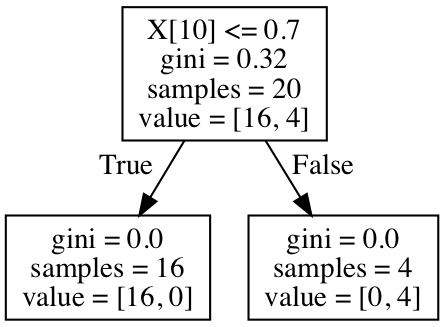
\includegraphics[scale=0.7]{graphs/tree_graph.png}
\label{fig:tree_graph}
\caption{\em Automatisierter Aufbau des Decision Tree durch \textit{sklearn} durch Prüfung der Merkmale}
\end{figure}

%\subsection{One-Class-Classification} \label{sec:oneclass}
%Die Wahl einer One-Class-Classification ist für die Diagnose einer möglichen ASS sehr gut geeignet. Die Funktionsweise des Klassifikators zur Detektion von Ausreißern entspricht der in dieser Arbeit getroffenen Problemstellung. 

%Die Evaluierung des entwickelten Algorithmus erfolgt mit Hilfe einer Kreuzvalidierung. Dies ermöglicht eine größtmögliche Statistik mit Hilfe der begrenzten Anzahl an gesammelten Daten. Bei der Entwicklung werden dabei zwei mögliche Klassifikations-Mechanismen durchgeführt. Zum einen einen Klassifikator mit $n$-Merkmalen sowie einem Ensemble von Klassifikatoren, welche unterschiedliche Klassifikationen durchführen und mit Hilfe eines zusätzlichen Klassifikators den zusammenfassenden und entscheidenden Mittelwert errechnet.

%Die in dieser Arbeit erreichten Ergebnisse sind dabei in Abbildung \ref{fig:eer_allinone} erkennbar. Hierbei ergibt sich für einen optimalen Threshold von $0.16$ einer Gleichfehlerrate (engl. \glqq Equal Error Rate\grqq{} (EER) von $20\%$. Die EER ermittelt dabei den Arbeitspunkt in dem die FMR und FNMR gleich sind.

%\begin{figure}[h!]
%\centering
%% This file was created by matplotlib2tikz v0.6.17.
\begin{tikzpicture}[scale=.8,transform shape]

\definecolor{color0}{rgb}{0.886274509803922,0.290196078431373,0.2}

\begin{axis}[
xlabel={FMR},
ylabel={FNMR},
xmin=0.01, xmax=1.16900119257737,
ymin=0.00488127212209496, ymax=1.28845678314721,
xmode=log,
ymode=log,
tick align=outside,
tick pos=left,
xmajorgrids,
x grid style={white!80.0!black},
ymajorgrids,
y grid style={white!80.0!black},
axis line style={white!80.0!black}
]
\addplot [semithick, color0, mark=*, mark size=3, mark options={solid}, forget plot]
table {%
0 1
0 1
0 1
0 0.962264150943396
0 0.880503144654088
0 0.849056603773585
0 0.779874213836478
0 0.735849056603774
0 0.723270440251572
0 0.635220125786163
0 0.559748427672956
0 0.534591194968553
0.0440251572327044 0.446540880503145
0.0754716981132075 0.415094339622641
0.132075471698113 0.345911949685535
0.169811320754717 0.257861635220126
0.207547169811321 0.20125786163522
0.226415094339623 0.106918238993711
0.251572327044025 0.0817610062893082
0.320754716981132 0.0628930817610063
0.421383647798742 0.0566037735849057
0.465408805031447 0.0377358490566038
0.522012578616352 0.0314465408805031
0.59748427672956 0.0314465408805031
0.660377358490566 0.0188679245283019
0.723270440251572 0.0125786163522013
0.748427672955975 0.00628930817610063
0.811320754716981 0.00628930817610063
0.842767295597484 0.00628930817610063
0.874213836477987 0
0.880503144654088 0
0.89937106918239 0
0.918238993710692 0
0.937106918238994 0
0.943396226415094 0
0.943396226415094 0
0.962264150943396 0
0.968553459119497 0
0.968553459119497 0
0.974842767295598 0
0.981132075471698 0
0.981132075471698 0
0.987421383647799 0
0.987421383647799 0
0.987421383647799 0
0.993710691823899 0
1 0
1 0
1 0
1 0
1 0
1 0
1 0
1 0
1 0
1 0
1 0
1 0
1 0
1 0
1 0
1 0
1 0
1 0
1 0
1 0
1 0
1 0
1 0
1 0
1 0
1 0
1 0
1 0
1 0
1 0
1 0
1 0
1 0
1 0
1 0
1 0
1 0
1 0
1 0
1 0
1 0
1 0
1 0
1 0
1 0
1 0
1 0
1 0
1 0
1 0
1 0
1 0
1 0
1 0
1 0
};
\end{axis}

\end{tikzpicture}
%\label{fig:eer_allinone}
%\caption{\em Der \glqq Decision-Error-Tradeoff\grqq{} (DET) zur Gegenüberstellung der FMR und FNMR}
%\end{figure}

\subsection{Support-Vector-Machine}
Da es sich bei der Problemstellung um eine Klassifikation von zwei statischen Klassen handelt, ist der Einsatz einer Support-Vector-Machine (SVM) denkbar. Besonders die große Dimension der Merkmalsvektoren ist hierbei ein Grund zur Wahl einer SVM. In dieser Arbeit werden dabei der \glqq Radial Basic Function\grqq{} (RBF) Kernel sowie eine SVM mit linearem Kernel verglichen.
Die in dieser Arbeit implementierte SVM wird mit Hilfe des Framework \textit{sklearn} umgesetzt. Um eine für die SVM möglichst aussagekräftige Statistik zu erhalten und die bestmöglichen Parameter zu ermitteln, erfolgt bei der Evaluation eine  Kreuzvalidierung. Zudem werden bei der Verwendung der \textit{sklearn}-SVM die Parameter $\gamma$ und $C$ variiert um ein Over- und Underfitting zu vermeiden.
Das Resultat zur Wahl der Parameter zeigt hierbei, dass bei einer Wahl des Paramaters $C=1$ und des zusätzlichen Parameters $\gamma = 0.0977$ für eine SVM mit RBF Kernel, bereits eine Genauigkeit (engl. \glqq Accuracy\grqq{} (ACC)) von ca. 99\% erreicht werden kann (siehe Abbildung \ref{fig:c_chooseSVM} und \ref{fig:gamma_chooseSVM}).

\begin{figure}[h!]
\centering
% This file was created by matplotlib2tikz v0.6.17.
\begin{tikzpicture}[scale=.8,transform shape]

\definecolor{color0}{rgb}{0.886274509803922,0.290196078431373,0.2}
\definecolor{color1}{rgb}{0.203921568627451,0.541176470588235,0.741176470588235}
\definecolor{color2}{rgb}{0.596078431372549,0.556862745098039,0.835294117647059}

\begin{axis}[
xlabel={Parameter C},
ylabel={Accuracy},
xmin=-0.05, xmax=1.05,
ymin=0.688172131147541, ymax=1.00969672131148,
tick align=outside,
tick pos=left,
xmajorgrids,
x grid style={white!80.0!black},
ymajorgrids,
y grid style={white!80.0!black},
axis line style={white!80.0!black},
legend entries={{Linear mit result},{RBF mit result},{Linear ohne result},{RBF ohne result}},
legend cell align={left},
legend style={at={(0.97,0.03)}, anchor=south east, draw=none}
]
\addplot [semithick, color0, mark=*, mark size=3, mark options={solid}]
table {%
1e-100 0.704426229508197
1.02353102189903e-99 0.704426229508197
1.04761575278967e-98 0.704426229508197
1.07226722201033e-97 0.704426229508197
1.09749876549306e-96 0.704426229508197
1.12332403297803e-95 0.704426229508197
1.14975699539774e-94 0.704426229508197
1.176811952435e-93 0.704426229508197
1.20450354025879e-92 0.704426229508197
1.23284673944207e-91 0.704426229508197
1.26185688306603e-90 0.704426229508197
1.29154966501489e-89 0.704426229508197
1.32194114846604e-88 0.704426229508197
1.35304777457982e-87 0.704426229508197
1.38488637139389e-86 0.704426229508197
1.41747416292682e-85 0.704426229508197
1.45082877849595e-84 0.704426229508197
1.48496826225448e-83 0.704426229508197
1.51991108295295e-82 0.704426229508197
1.55567614393049e-81 0.704426229508197
1.59228279334111e-80 0.704426229508197
1.62975083462067e-79 0.704426229508197
1.66810053720008e-78 0.704426229508197
1.70735264747072e-77 0.704426229508197
1.74752840000771e-76 0.704426229508197
1.78864952905746e-75 0.704426229508197
1.8307382802954e-74 0.704426229508197
1.87381742286042e-73 0.704426229508197
1.91791026167252e-72 0.704426229508197
1.96304065004031e-71 0.704426229508197
2.00923300256509e-70 0.704426229508197
2.05651230834869e-69 0.704426229508197
2.10490414451206e-68 0.704426229508197
2.15443469003193e-67 0.704426229508197
2.20513073990309e-66 0.704426229508197
2.25701971963397e-65 0.704426229508197
2.31012970008318e-64 0.704426229508197
2.36448941264543e-63 0.704426229508197
2.4201282647944e-62 0.704426229508197
2.47707635599173e-61 0.704426229508197
2.53536449397014e-60 0.704426229508197
2.59502421139976e-59 0.704426229508197
2.65608778294672e-58 0.704426229508197
2.71858824273297e-57 0.704426229508197
2.78255940220716e-56 0.704426229508197
2.84803586843584e-55 0.704426229508197
2.91505306282522e-54 0.704426229508197
2.98364724028338e-53 0.704426229508197
3.05385550883341e-52 0.704426229508197
3.12571584968823e-51 0.704426229508197
3.19926713779738e-50 0.704426229508197
3.27454916287773e-49 0.704426229508197
3.35160265093885e-48 0.704426229508197
3.43046928631493e-47 0.704426229508197
3.51119173421514e-46 0.704426229508197
3.59381366380464e-45 0.704426229508197
3.67837977182865e-44 0.704426229508197
3.76493580679249e-43 0.704426229508197
3.85352859371055e-42 0.704426229508197
3.94420605943768e-41 0.704426229508197
4.03701725859658e-40 0.704426229508197
4.13201240011537e-39 0.704426229508197
4.22924287438953e-38 0.704426229508197
4.3287612810831e-37 0.704426229508197
4.43062145758392e-36 0.704426229508197
4.53487850812863e-35 0.704426229508197
4.64158883361283e-34 0.704426229508197
4.75081016210285e-33 0.704426229508197
4.86260158006541e-32 0.704426229508197
4.97702356433218e-31 0.704426229508197
5.09413801481645e-30 0.704426229508197
5.21400828799976e-29 0.704426229508197
5.33669923120639e-28 0.704426229508197
5.46227721768442e-27 0.704426229508197
5.59081018251231e-26 0.704426229508197
5.72236765935031e-25 0.704426229508197
5.85702081805677e-24 0.704426229508197
5.99484250318952e-23 0.704426229508197
6.13590727341329e-22 0.704426229508197
6.28029144183437e-21 0.704426229508197
6.42807311728445e-20 0.704426229508197
6.57933224657582e-19 0.704426229508197
6.73415065775097e-18 0.704426229508197
6.89261210434985e-17 0.704426229508197
7.0548023107188e-16 0.704426229508197
7.22080901838563e-15 0.704426229508197
7.39072203352596e-14 0.704426229508197
7.56463327554648e-13 0.704426229508197
7.74263682681147e-12 0.704426229508197
7.92482898353938e-11 0.704426229508197
8.11130830789709e-10 0.704426229508197
8.30217568131997e-09 0.704426229508197
8.49753435908668e-08 0.704426229508197
8.69749002617809e-07 0.704426229508197
8.90215085445065e-06 0.704426229508197
9.11162756115517e-05 0.702786885245902
0.000932603346883218 0.85051912568306
0.00954548456661833 0.916256830601093
0.0977009957299225 0.977021857923497
1 0.995081967213115
};
\addplot [semithick, color1, mark=asterisk*, mark size=3, mark options={solid}]
table {%
1e-100 0.704426229508197
1.02353102189903e-99 0.704426229508197
1.04761575278967e-98 0.704426229508197
1.07226722201033e-97 0.704426229508197
1.09749876549306e-96 0.704426229508197
1.12332403297803e-95 0.704426229508197
1.14975699539774e-94 0.704426229508197
1.176811952435e-93 0.704426229508197
1.20450354025879e-92 0.704426229508197
1.23284673944207e-91 0.704426229508197
1.26185688306603e-90 0.704426229508197
1.29154966501489e-89 0.704426229508197
1.32194114846604e-88 0.704426229508197
1.35304777457982e-87 0.704426229508197
1.38488637139389e-86 0.704426229508197
1.41747416292682e-85 0.704426229508197
1.45082877849595e-84 0.704426229508197
1.48496826225448e-83 0.704426229508197
1.51991108295295e-82 0.704426229508197
1.55567614393049e-81 0.704426229508197
1.59228279334111e-80 0.704426229508197
1.62975083462067e-79 0.704426229508197
1.66810053720008e-78 0.704426229508197
1.70735264747072e-77 0.704426229508197
1.74752840000771e-76 0.704426229508197
1.78864952905746e-75 0.704426229508197
1.8307382802954e-74 0.704426229508197
1.87381742286042e-73 0.704426229508197
1.91791026167252e-72 0.704426229508197
1.96304065004031e-71 0.704426229508197
2.00923300256509e-70 0.704426229508197
2.05651230834869e-69 0.704426229508197
2.10490414451206e-68 0.704426229508197
2.15443469003193e-67 0.704426229508197
2.20513073990309e-66 0.704426229508197
2.25701971963397e-65 0.704426229508197
2.31012970008318e-64 0.704426229508197
2.36448941264543e-63 0.704426229508197
2.4201282647944e-62 0.704426229508197
2.47707635599173e-61 0.704426229508197
2.53536449397014e-60 0.704426229508197
2.59502421139976e-59 0.704426229508197
2.65608778294672e-58 0.704426229508197
2.71858824273297e-57 0.704426229508197
2.78255940220716e-56 0.704426229508197
2.84803586843584e-55 0.704426229508197
2.91505306282522e-54 0.704426229508197
2.98364724028338e-53 0.704426229508197
3.05385550883341e-52 0.704426229508197
3.12571584968823e-51 0.704426229508197
3.19926713779738e-50 0.704426229508197
3.27454916287773e-49 0.704426229508197
3.35160265093885e-48 0.704426229508197
3.43046928631493e-47 0.704426229508197
3.51119173421514e-46 0.704426229508197
3.59381366380464e-45 0.704426229508197
3.67837977182865e-44 0.704426229508197
3.76493580679249e-43 0.704426229508197
3.85352859371055e-42 0.704426229508197
3.94420605943768e-41 0.704426229508197
4.03701725859658e-40 0.704426229508197
4.13201240011537e-39 0.704426229508197
4.22924287438953e-38 0.704426229508197
4.3287612810831e-37 0.704426229508197
4.43062145758392e-36 0.704426229508197
4.53487850812863e-35 0.704426229508197
4.64158883361283e-34 0.704426229508197
4.75081016210285e-33 0.704426229508197
4.86260158006541e-32 0.704426229508197
4.97702356433218e-31 0.704426229508197
5.09413801481645e-30 0.704426229508197
5.21400828799976e-29 0.704426229508197
5.33669923120639e-28 0.704426229508197
5.46227721768442e-27 0.704426229508197
5.59081018251231e-26 0.704426229508197
5.72236765935031e-25 0.704426229508197
5.85702081805677e-24 0.704426229508197
5.99484250318952e-23 0.704426229508197
6.13590727341329e-22 0.704426229508197
6.28029144183437e-21 0.704426229508197
6.42807311728445e-20 0.704426229508197
6.57933224657582e-19 0.704426229508197
6.73415065775097e-18 0.704426229508197
6.89261210434985e-17 0.704426229508197
7.0548023107188e-16 0.704426229508197
7.22080901838563e-15 0.704426229508197
7.39072203352596e-14 0.704426229508197
7.56463327554648e-13 0.704426229508197
7.74263682681147e-12 0.704426229508197
7.92482898353938e-11 0.704426229508197
8.11130830789709e-10 0.704426229508197
8.30217568131997e-09 0.704426229508197
8.49753435908668e-08 0.704426229508197
8.69749002617809e-07 0.704426229508197
8.90215085445065e-06 0.704426229508197
9.11162756115517e-05 0.704426229508197
0.000932603346883218 0.704426229508197
0.00954548456661833 0.704426229508197
0.0977009957299225 0.935983606557377
1 0.981912568306011
};
\addplot [semithick, blue, dash pattern=on 1pt off 3pt on 3pt off 3pt]
table {%
1e-100 0.704426229508197
1.02353102189903e-99 0.704426229508197
1.04761575278967e-98 0.704426229508197
1.07226722201033e-97 0.704426229508197
1.09749876549306e-96 0.704426229508197
1.12332403297803e-95 0.704426229508197
1.14975699539774e-94 0.704426229508197
1.176811952435e-93 0.704426229508197
1.20450354025879e-92 0.704426229508197
1.23284673944207e-91 0.704426229508197
1.26185688306603e-90 0.704426229508197
1.29154966501489e-89 0.704426229508197
1.32194114846604e-88 0.704426229508197
1.35304777457982e-87 0.704426229508197
1.38488637139389e-86 0.704426229508197
1.41747416292682e-85 0.704426229508197
1.45082877849595e-84 0.704426229508197
1.48496826225448e-83 0.704426229508197
1.51991108295295e-82 0.704426229508197
1.55567614393049e-81 0.704426229508197
1.59228279334111e-80 0.704426229508197
1.62975083462067e-79 0.704426229508197
1.66810053720008e-78 0.704426229508197
1.70735264747072e-77 0.704426229508197
1.74752840000771e-76 0.704426229508197
1.78864952905746e-75 0.704426229508197
1.8307382802954e-74 0.704426229508197
1.87381742286042e-73 0.704426229508197
1.91791026167252e-72 0.704426229508197
1.96304065004031e-71 0.704426229508197
2.00923300256509e-70 0.704426229508197
2.05651230834869e-69 0.704426229508197
2.10490414451206e-68 0.704426229508197
2.15443469003193e-67 0.704426229508197
2.20513073990309e-66 0.704426229508197
2.25701971963397e-65 0.704426229508197
2.31012970008318e-64 0.704426229508197
2.36448941264543e-63 0.704426229508197
2.4201282647944e-62 0.704426229508197
2.47707635599173e-61 0.704426229508197
2.53536449397014e-60 0.704426229508197
2.59502421139976e-59 0.704426229508197
2.65608778294672e-58 0.704426229508197
2.71858824273297e-57 0.704426229508197
2.78255940220716e-56 0.704426229508197
2.84803586843584e-55 0.704426229508197
2.91505306282522e-54 0.704426229508197
2.98364724028338e-53 0.704426229508197
3.05385550883341e-52 0.704426229508197
3.12571584968823e-51 0.704426229508197
3.19926713779738e-50 0.704426229508197
3.27454916287773e-49 0.704426229508197
3.35160265093885e-48 0.704426229508197
3.43046928631493e-47 0.704426229508197
3.51119173421514e-46 0.704426229508197
3.59381366380464e-45 0.704426229508197
3.67837977182865e-44 0.704426229508197
3.76493580679249e-43 0.704426229508197
3.85352859371055e-42 0.704426229508197
3.94420605943768e-41 0.704426229508197
4.03701725859658e-40 0.704426229508197
4.13201240011537e-39 0.704426229508197
4.22924287438953e-38 0.704426229508197
4.3287612810831e-37 0.704426229508197
4.43062145758392e-36 0.704426229508197
4.53487850812863e-35 0.704426229508197
4.64158883361283e-34 0.704426229508197
4.75081016210285e-33 0.704426229508197
4.86260158006541e-32 0.704426229508197
4.97702356433218e-31 0.704426229508197
5.09413801481645e-30 0.704426229508197
5.21400828799976e-29 0.704426229508197
5.33669923120639e-28 0.704426229508197
5.46227721768442e-27 0.704426229508197
5.59081018251231e-26 0.704426229508197
5.72236765935031e-25 0.704426229508197
5.85702081805677e-24 0.704426229508197
5.99484250318952e-23 0.704426229508197
6.13590727341329e-22 0.704426229508197
6.28029144183437e-21 0.704426229508197
6.42807311728445e-20 0.704426229508197
6.57933224657582e-19 0.704426229508197
6.73415065775097e-18 0.704426229508197
6.89261210434985e-17 0.704426229508197
7.0548023107188e-16 0.704426229508197
7.22080901838563e-15 0.704426229508197
7.39072203352596e-14 0.704426229508197
7.56463327554648e-13 0.704426229508197
7.74263682681147e-12 0.704426229508197
7.92482898353938e-11 0.704426229508197
8.11130830789709e-10 0.704426229508197
8.30217568131997e-09 0.704426229508197
8.49753435908668e-08 0.704426229508197
8.69749002617809e-07 0.704426229508197
8.90215085445065e-06 0.704426229508197
9.11162756115517e-05 0.702786885245902
0.000932603346883218 0.85051912568306
0.00954548456661833 0.916256830601093
0.0977009957299225 0.977021857923497
1 0.995081967213115
};
\addplot [semithick, color2, mark=x, mark size=3, mark options={solid}]
table {%
1e-100 0.704426229508197
1.02353102189903e-99 0.704426229508197
1.04761575278967e-98 0.704426229508197
1.07226722201033e-97 0.704426229508197
1.09749876549306e-96 0.704426229508197
1.12332403297803e-95 0.704426229508197
1.14975699539774e-94 0.704426229508197
1.176811952435e-93 0.704426229508197
1.20450354025879e-92 0.704426229508197
1.23284673944207e-91 0.704426229508197
1.26185688306603e-90 0.704426229508197
1.29154966501489e-89 0.704426229508197
1.32194114846604e-88 0.704426229508197
1.35304777457982e-87 0.704426229508197
1.38488637139389e-86 0.704426229508197
1.41747416292682e-85 0.704426229508197
1.45082877849595e-84 0.704426229508197
1.48496826225448e-83 0.704426229508197
1.51991108295295e-82 0.704426229508197
1.55567614393049e-81 0.704426229508197
1.59228279334111e-80 0.704426229508197
1.62975083462067e-79 0.704426229508197
1.66810053720008e-78 0.704426229508197
1.70735264747072e-77 0.704426229508197
1.74752840000771e-76 0.704426229508197
1.78864952905746e-75 0.704426229508197
1.8307382802954e-74 0.704426229508197
1.87381742286042e-73 0.704426229508197
1.91791026167252e-72 0.704426229508197
1.96304065004031e-71 0.704426229508197
2.00923300256509e-70 0.704426229508197
2.05651230834869e-69 0.704426229508197
2.10490414451206e-68 0.704426229508197
2.15443469003193e-67 0.704426229508197
2.20513073990309e-66 0.704426229508197
2.25701971963397e-65 0.704426229508197
2.31012970008318e-64 0.704426229508197
2.36448941264543e-63 0.704426229508197
2.4201282647944e-62 0.704426229508197
2.47707635599173e-61 0.704426229508197
2.53536449397014e-60 0.704426229508197
2.59502421139976e-59 0.704426229508197
2.65608778294672e-58 0.704426229508197
2.71858824273297e-57 0.704426229508197
2.78255940220716e-56 0.704426229508197
2.84803586843584e-55 0.704426229508197
2.91505306282522e-54 0.704426229508197
2.98364724028338e-53 0.704426229508197
3.05385550883341e-52 0.704426229508197
3.12571584968823e-51 0.704426229508197
3.19926713779738e-50 0.704426229508197
3.27454916287773e-49 0.704426229508197
3.35160265093885e-48 0.704426229508197
3.43046928631493e-47 0.704426229508197
3.51119173421514e-46 0.704426229508197
3.59381366380464e-45 0.704426229508197
3.67837977182865e-44 0.704426229508197
3.76493580679249e-43 0.704426229508197
3.85352859371055e-42 0.704426229508197
3.94420605943768e-41 0.704426229508197
4.03701725859658e-40 0.704426229508197
4.13201240011537e-39 0.704426229508197
4.22924287438953e-38 0.704426229508197
4.3287612810831e-37 0.704426229508197
4.43062145758392e-36 0.704426229508197
4.53487850812863e-35 0.704426229508197
4.64158883361283e-34 0.704426229508197
4.75081016210285e-33 0.704426229508197
4.86260158006541e-32 0.704426229508197
4.97702356433218e-31 0.704426229508197
5.09413801481645e-30 0.704426229508197
5.21400828799976e-29 0.704426229508197
5.33669923120639e-28 0.704426229508197
5.46227721768442e-27 0.704426229508197
5.59081018251231e-26 0.704426229508197
5.72236765935031e-25 0.704426229508197
5.85702081805677e-24 0.704426229508197
5.99484250318952e-23 0.704426229508197
6.13590727341329e-22 0.704426229508197
6.28029144183437e-21 0.704426229508197
6.42807311728445e-20 0.704426229508197
6.57933224657582e-19 0.704426229508197
6.73415065775097e-18 0.704426229508197
6.89261210434985e-17 0.704426229508197
7.0548023107188e-16 0.704426229508197
7.22080901838563e-15 0.704426229508197
7.39072203352596e-14 0.704426229508197
7.56463327554648e-13 0.704426229508197
7.74263682681147e-12 0.704426229508197
7.92482898353938e-11 0.704426229508197
8.11130830789709e-10 0.704426229508197
8.30217568131997e-09 0.704426229508197
8.49753435908668e-08 0.704426229508197
8.69749002617809e-07 0.704426229508197
8.90215085445065e-06 0.704426229508197
9.11162756115517e-05 0.704426229508197
0.000932603346883218 0.704426229508197
0.00954548456661833 0.704426229508197
0.0977009957299225 0.932650273224044
1 0.981912568306011
};
\end{axis}

\end{tikzpicture}
\label{fig:c_chooseSVM}
\caption{\em Wahl des Parameter C mit Hilfe einer Kreuzvalidierung für eine SVM mit linearem und RBF Kernel}
\end{figure}

\begin{figure}[h!]
\centering
% This file was created by matplotlib2tikz v0.6.17.
\begin{tikzpicture}[scale=.8,transform shape]

\definecolor{color0}{rgb}{0.886274509803922,0.290196078431373,0.2}
\definecolor{color1}{rgb}{0.203921568627451,0.541176470588235,0.741176470588235}

\begin{axis}[
xlabel={Parameter $\gamma$},
ylabel={Accuracy},
xmin=2.84803586843589e-10, xmax=2.8480358684358,
ymin=0.690468579234973, ymax=1.0,
xmode=log,
tick align=outside,
tick pos=left,
xmajorgrids,
x grid style={white!80.0!black},
ymajorgrids,
y grid style={white!80.0!black},
axis line style={white!80.0!black},
legend entries={{RBF mit result},{RBF ohne result}},
legend cell align={left},
legend style={at={(0.03,0.97)}, anchor=north west, draw=none}
]
\addplot [semithick, color0, mark=asterisk*, mark size=3, mark options={solid}]
table {%
8.11130830789709e-10 0.704426229508197
8.30217568131997e-09 0.704426229508197
8.49753435908668e-08 0.704426229508197
8.69749002617809e-07 0.704426229508197
8.90215085445065e-06 0.704426229508197
9.11162756115517e-05 0.704426229508197
0.000932603346883218 0.704426229508197
0.00954548456661833 0.96551912568306
0.0977009957299225 0.983579234972678
1 0.942540983606558
};
\addplot [semithick, color1, mark=x, mark size=3, mark options={solid}]
table {%
8.11130830789709e-10 0.704426229508197
8.30217568131997e-09 0.704426229508197
8.49753435908668e-08 0.704426229508197
8.69749002617809e-07 0.704426229508197
8.90215085445065e-06 0.704426229508197
9.11162756115517e-05 0.704426229508197
0.000932603346883218 0.704426229508197
0.00954548456661833 0.963879781420765
0.0977009957299225 0.983579234972678
1 0.942540983606558
};
\end{axis}

\end{tikzpicture}
\label{fig:gamma_chooseSVM}
\caption{\em Wahl des Parameter $\gamma$ mit Hilfe einer Kreuzvalidierung für eine SVM mit linearem und RBF Kernel}
\end{figure}

\subsection{K-Nearest-Neighbour} \label{sec:kneighbour}
Neben der Support-Vector-Machine dient der Algorithmus K-Nearest-Neighbour ebenso sehr gut zur Detektion von Ausreißern. In diesem Algorithmus ist es möglich nicht nur Ausreißer zu erkennen sondern auch eine Unterscheidung innerhalb der zwei Klassen einer diagnostizierten ASS und einer nicht diagnostizierten ASS durchzuführen. Innerhalb des Algorithmus wird neben der Distanz zu den Nachbarn ebenso die Anzahl der $k$ nächsten Nachbarn variiert.
Das Ergebnis des Algorithmus zeigt dabei nach Abbildung \ref{fig:k_neighbours}, dass bei einer Anzahl von $k=15$ Nachbarn für den Datensatz mit dem Merkmal \textit{result} eine Trennschärfe von 99\% erreicht werden kann. Im Vergleich dazu erreicht der Algorithmus ohne das Merkmal \textit{result} mit der Wahl $k=20$ eine Trennschärfe von 96\%. Die bessere Trennschärfe bei der Verwendung des zusätzlichen Merkmals ist dabei auf das Ergebnis aus der Datenanalyse zurückzuführen.

\begin{figure}[h!]
\centering
% This file was created by matplotlib2tikz v0.6.17.
\begin{tikzpicture}[scale=.8,transform shape]

\begin{axis}[
xlabel={Parameter K},
ylabel={Accuracy},
xmin=-0.4, xmax=30.4,
ymin=0.92975, ymax=0.994758196721311,
tick align=outside,
tick pos=left,
xmajorgrids,
x grid style={white!80.0!black},
ymajorgrids,
y grid style={white!80.0!black},
axis line style={white!80.0!black},
legend entries={{Mit result},{Ohne result}},
legend cell align={left},
legend style={at={(0.97,0.03)}, anchor=south east, draw=none}
]
\addplot [semithick, blue, mark=*, mark size=3, mark options={solid}]
table {%
1 0.947404371584699
2 0.940901639344262
3 0.947404371584699
4 0.952349726775956
5 0.955601092896175
6 0.96551912568306
7 0.968770491803279
8 0.970437158469945
9 0.975355191256831
10 0.972103825136612
11 0.977021857923497
12 0.983579234972678
13 0.983579234972678
14 0.988524590163934
15 0.988524590163934
16 0.991803278688524
17 0.990163934426229
18 0.991803278688524
19 0.991803278688524
20 0.990163934426229
21 0.991803278688524
22 0.990163934426229
23 0.991803278688524
24 0.990163934426229
25 0.990163934426229
26 0.990163934426229
27 0.990163934426229
28 0.986885245901639
29 0.988524590163934
};
\addplot [semithick, red, mark=x, mark size=3, mark options={solid}]
table {%
1 0.944125683060109
2 0.932704918032787
3 0.934262295081967
4 0.947404371584699
5 0.940846994535519
6 0.95568306010929
7 0.967131147540984
8 0.965491803278688
9 0.957295081967213
10 0.965546448087432
11 0.967158469945355
12 0.968825136612022
13 0.970464480874317
14 0.973743169398907
15 0.970464480874317
16 0.972103825136612
17 0.973743169398907
18 0.977049180327869
19 0.975382513661202
20 0.980327868852459
21 0.978661202185792
22 0.978688524590164
23 0.977049180327869
24 0.973770491803279
25 0.973770491803279
26 0.977049180327869
27 0.975409836065574
28 0.975382513661202
29 0.980327868852459
};
\end{axis}

\end{tikzpicture}
\label{fig:k_neighbours}
\caption{\em Errechnete Fehlerraten unter der Variation der Anzahl der Nachbarn}
\end{figure}

\subsection{K-Means}
Der Algorithmus K-Means ermittelt eine Fixpunkt von Vektoren und entspricht dabei dem Mittelwertsvektor $\vec{k_m}$ der trainierten Vektoren. Die Evaluation und Detektion der Ausreißer geschieht hierbei wie bereits in Abschnitt \ref{sec:kneighbour} beschrieben. Dabei werden die Anzahl der $k$ Merkmalsvektoren sowie die maximal mögliche Distanz zum Mittelwertsvektor $\vec{k_m}$ variiert.
Die Resultate des K-Means zeigen ....

\subsection{Evaluation der Algorithmen} \label{sec:evaluation}
Die Ergebnisse der angewandten Algorithmen zeigen für die Problemstellung stets eine gute Trennschärfe (siehe Tabelle \ref{tbl:results_table_without} und \ref{tbl:results_table}). Die Ergebnisse aus der vorangegangenen Datenanalyse zeigten bereits eine eindeutige Lösung des Datensatzes bezüglich der Klassifizierung der Daten. Aus diesem Grund wird in der Evaluation der Ergebnisse darauf geachtet, die Auswertung mit und ohne dem Merkmal \textit{result} durchzuführen.

\begin{table}[htbp]
\begin{tabular}{l c c c}
\textbf{Algorithmus} & \textbf{ACC} & \textbf{TPR} & \textbf{FPR} \\ \hline
Decision Tree & 92.2\% & 85.0\% & 14.9\% \\
lineare SVM & 95.0\% & 95.1\% & 4.8\% \\
RBF SVM & 97.8\% & 95.8\% & 4.1\% \\
K Nearest Neighbour & 96.9\% & 93.0\% & 6.9\%\\ 
K Means & 96.9\% & 93.0\% & 6.9\%\\ 
\end{tabular}
\centering
\label{tbl:results_table_without}
\caption{\em Die Resultate angewandten Algorithmen ohne das Merkmal \glqq result\grqq}
\end{table}

\begin{table}[htbp]
\begin{tabular}{l c c c}
\textbf{Algorithmus} & \textbf{ACC} & \textbf{TPR} & \textbf{FPR} \\ \hline
Decision Tree & 100\% & 100\% & 0\% \\
lineare SVM & 98.5\% & 98.2\% & 1.7\% \\
RBF SVM & 98.1\% & 100\% & 0\% \\
K Nearest Neighbour & 99.1\% & 96.7\% & 3.0\%\\ 
K Means & 99.1\% & 96.7\% & 3.0\%\\ 
\end{tabular}
\centering
\label{tbl:results_table}
\caption{\em Die Resultate angewandten Algorithmen inkl. dem Merkmal \glqq result\grqq}
\end{table}


\section{Fazit und Ausblick}
Anhand der Ergebnisse aus Kapitel \ref{sec:algorithms} lässt sich die Möglichkeit des Einsatzes von maschinellen Lernmethoden zur Diagnose von ASS bestätigen. Es können dabei durch die Anwendung eines geeigneten Algorithmus sehr gute Ergebnisse zur Tendenz einer Diagnose ermittelt werden. Diese können dabei dem behandelnden Arzt eine objektive Sichtweise der Bewertung des Verhaltens ermöglichen. Da der verwendete Datensatz von \textsc{Thabtah} \cite{Thabtah2017, Thabtah, Thabtah2018} jedoch bereits normierte Antworten enthält kann die Gewichtung der Antwort zur Analyse des Verhaltens nicht mit einbezogen werden. Ebenso enthalten die Datensätze eine Klassifizierung nach dem Vorgaben von \textsc{NICE} \cite{NICE2012}, welche die Problemstellung bereits vereinfacht löst (siehe Abschnitt \ref{sec:analysis} und \ref{sec:tree}). Abschließend lässt sich dennoch bestätigen, dass der unterstützende Einsatz von Methoden des maschinellen Lernens in der Diagnose mit sehr guten Ergebnissen möglich ist.

\printbibliography

\end{document}
